\subsection{Mayan Counting System}


\content{
        The Mayans were perhaps the most advanced civilizations of the ancient
        world. They had a sophisticated ritual system developed by a class of
        priests, which held time as divine and eternal. That being so, the
        calendar, and calculations related to it, were very important to them. 

        There were two numeral systems that the Mayans had, one used by priests
        and one used for day-to-day calculations. For the priests, the number
        system was governed by ritual, the days of the year were thought to be
        gods, so the formal symbols for the days were decorated heads, like the
        one below. 

        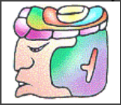
\includegraphics[scale=0.65]{mayan.png}

        We're not going to study this one. 
}{% presentation
}{% nopresentation
}{% comments
}

\content{
        The other system they used was a base 20 positional system. The symbols
        they used were as follows: 

        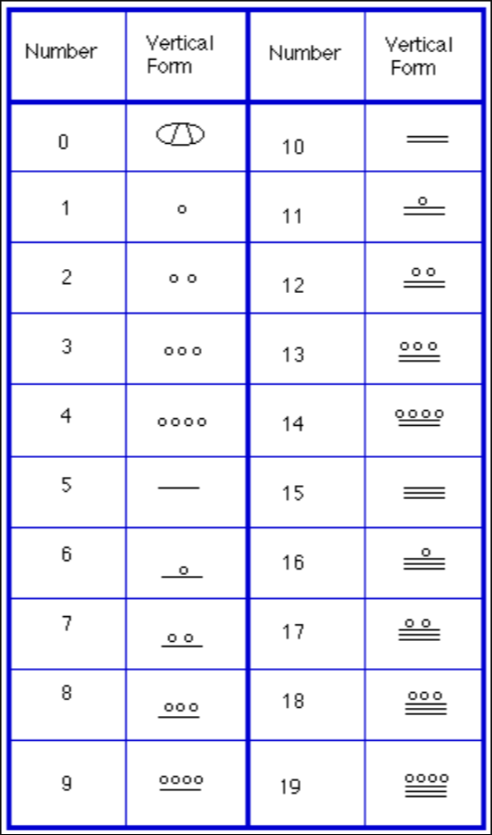
\includegraphics[scale=0.3]{mayan-symbols.png}
}{% presentation
}{% nopresentation
}{% comments
}

\content{
        Convert 1024 to the mayan base 20 system. 
}{% presentation
\vspace{3in}
}{% nopresentation
\vspace{3in}
}{% comments
}

\content{
        Convert 734 to the mayan base 20 system.
}{% presentation
\vspace{3in}
}{% nopresentation
\vspace{3in}
}{% comments
}

\content{
        Convert 192 to the mayan base 20 system.
}{% presentation
\vspace{3in}
}{% nopresentation
\vspace{3in}
}{% comments
}


\content{
        Compute 734 + 192 in the mayan base 20 system (use the conversions
        above).
}{% presentation
\vspace{3in}
}{% nopresentation
\vspace{3in}
}{% comments
}

\content{
        Compute 1028 + 734 in the mayan base 20 system (use the conversions
        above).
}{% presentation
\vspace{3in}
}{% nopresentation
\vspace{3in}
}{% comments
}
